\section{Rede Neural similar ao modelo de Holley e Karplus}

O modelo original de Holley e Karplus \citeyear{key} utilizava dois neurônios na camada oculta. Posteriormente, Chandonia e Karplus \citeyear{10.1002/pro.5560050422} aumentaram o conjunto de dados de 62 para 318 proteínas e observaram que um aumento da camada oculta de 2 para 8 neurônios produzia um aumento da acurácia de 63\% para 67\%.

\begin{figure}
    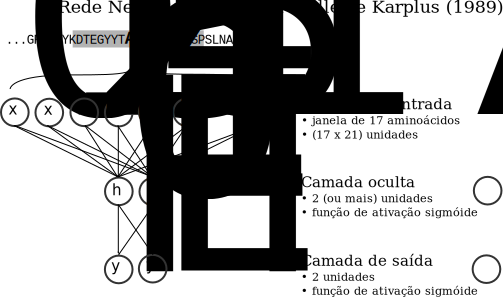
\includegraphics[width=\linewidth]{../figures/neural_network_HK.pdf}
    \caption{Rede neural utilizada nos trabalhos de Holley e Karplus \citeyear{key} e Chandonia e Karplus \citeyear{10.1002/pro.5560050422}. A rede neural utiliza como entrada uma janela de 17 aminoácidos da proteína, cada um codificado em um vetor de tamanho 21 (20 aa + 1 posição que indica ausência de aminoácidos). Na camada oculta foram testadas várias configurações, diferindo entre si pelo número de neurônios. A camada de saída possuía 2 neurônios, um representando a saída para hélice e outro para fitas. Todos os neurônios possuiam funções de ativação sigmóide. Os rótulos de treinamento foram $(1,0) \rightarrow hélice$, $(0,1) \rightarrow fita$, $(0,0) \rightarrow coil$.}
    \label{fig:neural_network_HK}
\end{figure}

Para avaliarmos qual seria o desempenho de uma rede neural com topologia similar a proposta por Holley e Karplus \citeyear{key} nós implementamos algumas redes neurais utilizando o framework Pytorch e treinamos com o conjunto de proteínas utilizado ao longo desse trabalho.

\begin{figure}
    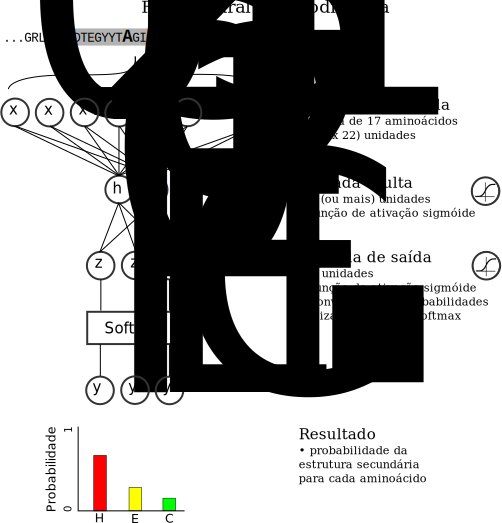
\includegraphics[width=\linewidth]{../figures/neural_network_HK_similar.pdf}
    \caption{Rede neural similar à utilizada no trabalho de Holley e Karplus \citeyear{key}. A principal diferença encontra-se na camada de saída onde foram utilizados 3 neurônios, ao invés de 2, cada um representando uma estrutura secundária. Em seguida, os valores dos neurônios passam por uma função Softmax para que a somatória das saídas seja igual a 1 assim, a saída representa a probabilidade da estrutura secundária para cada aminoácido. Os rótulos }
    \label{fig:neural_network_HK_similar}
\end{figure}